\section{Belgian Grand prix}

\subsection{Circuit Analysis}

\textbf{Circuit Name:} Circuit de Spa-Francorchamps (Stavelot, Belgium) \\
\textbf{Length:} 7.004 km - \textbf{Laps:} 44 - \textbf{Total Distance:} 308.052 km

\begin{figure}[H]
    \centering
    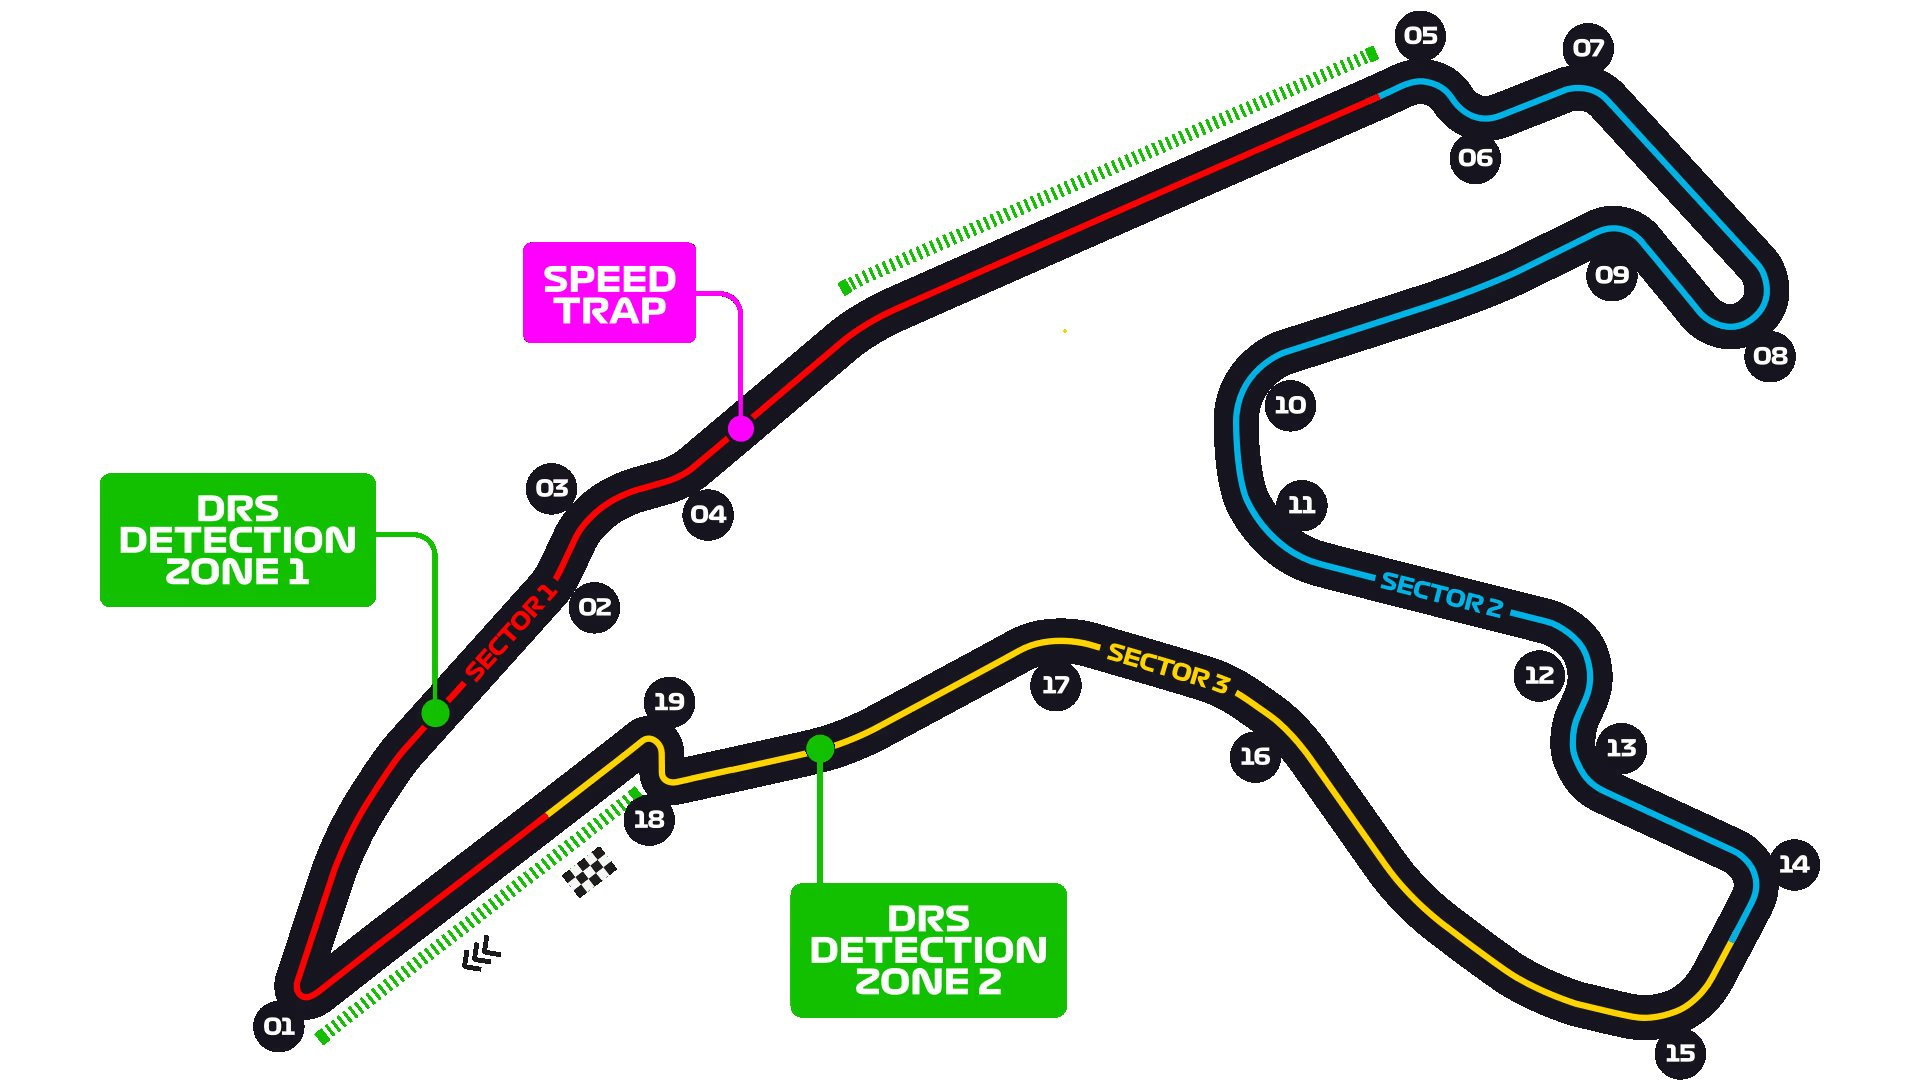
\includegraphics[width=0.75\linewidth]{images/14.Belgium_Circuit.jpg}
\end{figure}


\begin{itemize}
    \item \textbf{Lap Record} : 1:41.252 (2020, Lewis Hamilton – Mercedes).
    
    \item \textbf{Number of Corners \& Key Features} : 19 turns (10 right, 9 left). \\
    Iconic corners include Eau Rouge–Raidillon, Pouhon, and Blanchimont. High-speed circuit with major elevation changes.
    
    \item \textbf{Braking Zones \& Traction} : Heavy braking at La Source (Turn 1), Les Combes (Turn 5), and the Bus Stop chicane (Turns 18–19). \\
    Traction critical at exits of La Source and Turn 1 leading to long acceleration phases.
    
    \item \textbf{DRS \& Overtaking} : Two DRS zones (Kemmel straight, start/finish straight). \\
    Overtaking opportunities primarily at Les Combes and the Bus Stop chicane.
    
    \item \textbf{Tyre Degradation \& Strategy} : Medium degradation, with high lateral loads stressing tyres through fast corners. \\
    Two-stop strategies typical, but a one-stop can be attempted if conditions allow.
    
    \item \textbf{Weather \& Environment} : Famous for unpredictable Ardennes weather. \\
    Sudden showers possible, creating mixed conditions across different sectors of the track.
\end{itemize}

\textbf{Strategic Summary :} Spa demands aerodynamic efficiency, straight-line speed, and tyre management. Overtaking is more feasible than most tracks, but weather and Safety Cars often dictate race outcomes.

\subsection{Race Analysis}
\textbf{Date:} 28 July 2024 — 15:00 local time

\begin{itemize}
    \item \textbf{Qualifying Summary} : \textbf{Pole Position:} Charles Leclerc – 1:53.754. \\
    \textbf{Fastest lap in Q3:} Max Verstappen (Red Bull) – 1:53.159. \\
    Grid: Leclerc 1st, Pérez 2nd, Hamilton 3rd, Norris 4th.\\
    Max Verstappen, who finished 1st during the qualifications, was penalised of ten grid places for changing propulsion system components outside the quota.
    
    \item \textbf{Race Summary} : \textbf{Winner:} Lewis Hamilton (Mercedes) — back-to-back win after Hungary podium. \\
    \textbf{Podium:} 1. Hamilton - 2. Piastri - 3. Leclerc. \\
    Verstappen recovered from P11 to P4. \\
    Russell initially P1 but later disqualified for car underweight.\\
    
    \item \textbf{Strategies} : A race of fine margins under variable Spa weather. \\
    - Mercedes: Hamilton executed Medium–Hard–Medium, managing tyre wear superbly. Russell ran aggressive Medium–Medium–Hard, leading laps before DSQ. \\
    - McLaren: Piastri mirrored Hamilton’s Medium–Hard–Medium and almost stole victory on fresher tyres in final laps. Norris ran Medium–Hard–Medium as well, finishing P5. \\
    - Ferrari: Leclerc P3 (Medium–Hard–Medium), steady but lacked pace to fight Hamilton/Piastri. Sainz P6 with Medium–Hard–Hard. \\
    - Red Bull: Verstappen Medium–Hard–Hard, fast recovery drive but hindered by traffic. Pérez started P2, faded with tyre wear (P7) but took fastest lap. \\
    - Aston Martin: Alonso P8 and Stroll P11, both on Medium–Hard. \\
    - Alpine: Ocon P9, Gasly P13, solid midfield points. \\
    - Racing Bulls: Ricciardo P10, Tsunoda P16 — consistent but off the pace.
    
    \item \textbf{Performance Trends} : \textbf{Mercedes} showed their strongest pace of 2024, Hamilton mastering Spa’s conditions. \\
    \textbf{McLaren} were highly competitive, Piastri nearly winning. \\
    \textbf{Ferrari} consistent but again short of outright victory. \\
    \textbf{Red Bull} compromised by grid penalties and weak race execution — Verstappen only P4, Pérez P7. \\
    \textbf{Midfield}: Alpine and Aston Martin snatched points, Haas and Kick Sauber anonymous.
    
    \item \textbf{Championship Impact} : \textbf{Drivers:} Verstappen 277, Norris 199, Leclerc 177. \\
    \textbf{Constructors:} Red Bull 408, McLaren 366, Ferrari 345, Mercedes 266.
\end{itemize}

\textbf{Key Takeaway :} Hamilton triumphed at Spa thanks to perfect tyre management and strategy, resisting a late charge from Piastri. Ferrari showed consistency, while Red Bull’s struggles from poor grid positions limited their damage control.


\subsection{Link \& Takeaway}

\begin{itemize}
    \item Spa’s long straights and mixed-weather traits rewarded Mercedes’ strong balance and Hamilton’s experience. 
    \item McLaren’s race pace was excellent, with Piastri nearly stealing the win in the final laps. 
    \item Ferrari matched expectations with stable tyre life but lacked ultimate pace to challenge for victory. 
    \item Red Bull’s vulnerability from grid penalties showed how track position and execution are crucial at Spa. 
\end{itemize}